    \begin{table}
        \centering
        \begin{tabular}{lc|l|l|l|l|l|l}
            &&\multicolumn{5}{c}{\bf Number of Partitions}\\
            &&{\bf 2}&{\bf 4}&{\bf 8}&{\bf 16}&{\bf 32}\\
            \hline
            \multirow{5}{*}{\begin{sideways}{\bf Imbalance (\%)}\end{sideways}}
            &{\bf 5}&1036&1520&1818&1993&2087\\
            &{\bf 10}&1045&1495&1809&1987&2085\\
            &{\bf 15}&1031&1481&1798&1981&2097\\
            &{\bf 20}&1000&1482&1787&1971&2090\\
            &{\bf 25}&986&1464&1777&1965&2085\\
        \end{tabular}
        \caption[]{\label{tbl:hmetis} Number of cells to remove in order to fully partition the network, such that no users from one partition can communicate with any user in another partition. Columns indicate the number of desired partitions, and rows indicate the allowed imbalance between the largest partition and the average size (so for imbalance 5\%, k partitions, and n cells a partition cannot be more than $1.05 * \frac{n}{k}$). There are 2536 total hyperedges.}
    \end{table}
        
    Turning to our final goal, analysis of worst-case scenarios, we attend to two questions. 
    First, how much physical disaster would be required to fully partition the network?         
    Second, are there regional bottlenecks in the physical connectivity graph?

    \subsubsection*{Network Partitioning}
    We whimsically address an action-movie style disaster with the first question: how many physical disasters would it take for half of all prefixes to be in one partition, and half of all prefixes to be in another, such that no users in one partition can speak to the users in another partition?
    While the question is somewhat outrageous, the answer illuminates the redundancy of geographic connectivity across the globe, as we find that minimum cuts across our regional connectivity graph are quite large.
    
    To address this question, we use the {\tt hmetis} software package~\cite{hmetis} to discover balanced graph cuts.
    {\tt hmetis} performs hypergraph partitioning to discover minimum cuts that leave behind a balanced number of vertices on either side of the cut.
    We provided {\tt hmetis} with vertices for each AS, and hyperedges for each cell connecting all ASes which peer in that cell. 
    We then weighted each AS with the number of prefixes it announces, using origin prefix data from iPlane~\cite{iplane}.
    This is an overestimate of connectivity, as it clusters together all ASes which peer in the same region, even though those ASes may not all peer with each other in that region.
 
    Table~\ref{tbl:hmetis} displays the number of hyperedges (cells) whose removal was required to partition the network into  2, 4, 8, or 16 approximately equal sized cuts. 
    The rows of the table indicate the allowed imbalance in size between the partitions, the percent imbalance permissible between the largest partition and the average sized partition.
    We observe that even when imbalance is generous and the partitioning is only into two halves, 986 cells must be cut from the world map.
    This illustrates how tightly the global AS-connectivity graph is bound - there is no division of prefixes such that a cut is easy.
    Given a disaster event that could achieve such a cut would have much more significant impacts on other aspects of society, we are forced to conclude that any action-movie that considers this scenario will not focus on the impact to interdomain connectivity.
    
    \subsubsection*{Regional Bottlenecks}
    We now turn to a more practical question of recent political interest: regional bottlenecks in connectivity.
    Recent events in Iran~\cite{iran}, Egypt~\cite{egypt}, and China~\cite{china} exemplify the implications of the fact that each nation's connectivity to the outside world traverses one or a handful of egress points.
    This leaves the countries vulnerable to malicious or accidental failure at these bottlenecks.
    We seek to identify regions which are similarly vulnerable, by once again examining our regional connectivity graph. 
    Specifically, we seek to identify regions that could be isolated from the rest of the Internet due to a disaster that disables some number of cells in which ASes interconnect; we refer to this number as the `budget' of such a cut.

    In order to answer this question, we must first determine the geographic extent of end-hosts served by an AS.
    For each AS, we take a random sampling of IP addresses from the announced prefixes seen in the BGP tables provided by the Routeviews project~\cite{routeviews}. 
    We then geolocate each IP address using the MaxMind database, and map each IP address to a hexagonal grid cell in the same manner as we did for AS interconnection locations.
    Finally, we cluster together cells that lie within a distance threshold of each other, and repeatedly merge these clusters closer than that same distance threshold together until we reach convergence.
    Given this sampling of cells, we define the geographic extent of an AS to be the area within the convex hull around each of these clusters. 
    Because we only consider non-stub ASes, we add the extent of all stub ASes to that of each of their providers.
    In particular, the extent of a multihomed stub AS is added to that of all of its providers.

    Once we have determined both the geographic extent of each AS, as well as the locations in which each AS interconnects, we can easily determine regions of Earth that could be isolated by removing a given budget of interconnection cells.
    A cell is vulnerable to being isolated if it is served only by ASNs which interconnect in fewer unique places than our budget.

    % need a map that shows color coded "vulnerable" regions. 3, 10, 100, 1000.
    \begin{figure}[tb]
\centering
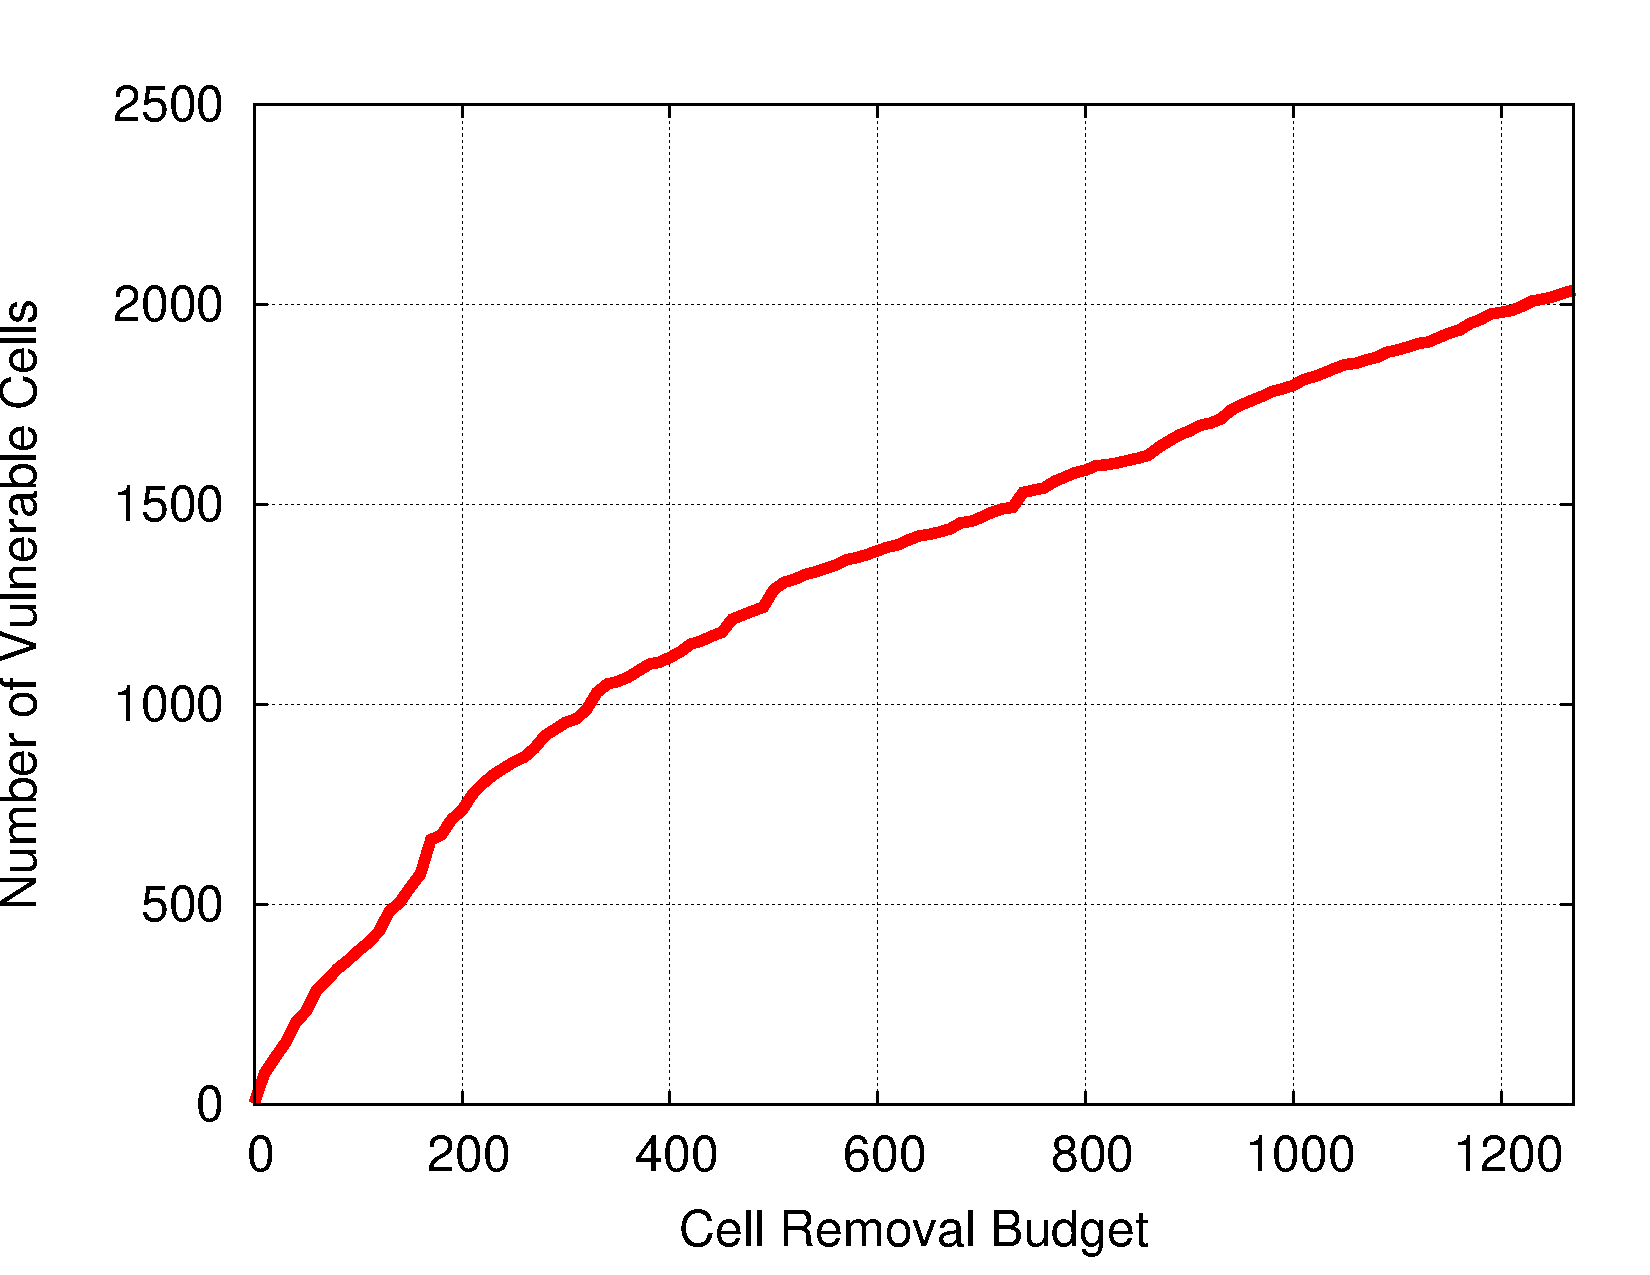
\includegraphics[width=3.25in]{isolation}
\caption[]{\label{fig:isolation} Number of cells potentially isolated given a budget of cells containing AS interconnections to remove. As expected, the trend is generally increasing, though isolating more nodes becomes increasingly more difficult as the budget increases.} 
\end{figure}

    We find that for modest budgets (ten or fewer) relatively few cells are in danger of being isolated.
    The relationship between budget and number of potentially isolated cells is seen in Figure~\ref{fig:isolation}. 
    However, due to the poor quality of our geolocation of interconnection points, it is likely that interconnection points are more concentrated than we assume for our model.
    As a result, the actual number of vulnerable regions could be much higher at these low budgets.

    We can consider higher budget scenarios to compensate for this error. 
    When we consider a budget of 500 removed interconnection points, we find 1286 potentially vulnerable cells. 
    These cells cover primarily non-urban areas and islands.
    Interestingly, all of the Philippines appear vulnerable at this budget level, as do significant portions of Iran and Turkey. 

    This analysis is, necessarily, incomplete.
    Improved geolocation accuracy for core routers and better coverage for end hosts outside the US and Europe would greatly improve our ability to identify regions at risk of isolation. 
    Nevertheless, it suggests that there are regions that suffer bottlenecks in their physical connectivity and thus may be at significant risk in the event of a regional-scale disaster. 
